\documentclass[a4paper,12pt]{article}

\usepackage[russian]{babel}
\usepackage{cmap}
\usepackage[utf8]{inputenc}
\usepackage[usenames]{color}
\usepackage{tabularray}
\usepackage{xcolor}
\usepackage{graphicx} 
\usepackage{subfigure}
\usepackage{subcaption}

\usepackage[unicode]{hyperref} % цвета гиперссылок
\hypersetup{
	colorlinks,
	citecolor=black,
	filecolor=black,
	linkcolor=blue,
	urlcolor=black
}

\usepackage{geometry} % задаёт поля 
%\geometry{left=3cm}
%\geometry{right= 1.5cm}
%\geometry{top=2cm}
%\geometry{bottom=2cm} 

\usepackage{enumitem} % настраивает работу со списками:
\def\labelitemi{—} % ... задаёт длинное тире как стандартный маркер ненумерованного списка
\setlist{nolistsep} %  ... убирает дополнительный отступы между элементами списка


% удаляет названия и продолжение следует и т. для таблиц, будет только таблица без всего
\DefTblrTemplate{contfoot-text}{default}{}
\DefTblrTemplate{conthead-text}{default}{}
\DefTblrTemplate{caption}{default}{}
\DefTblrTemplate{conthead}{default}{}
\DefTblrTemplate{capcont}{default}{}


\title{Повышение эффективности\\ регрессионных моделей за счет исключения аномальных данных}
\author{В. Г. Мосин}
\date{}

%   \input{preamble.tex}
\begin{document}
	\maketitle
	\abstract{\noindent  Исследован метод, определяющий влияние выбросов на производительность регрессионных моделей. На примере данных о потреблении контента одного из ведущих хостингов показано, что исключение аномальных объектов способно существенно повысить их прогнозирующую способность. Даны рекомендации по применению метода исключения аномальных данных.}
	
\tableofcontents
	
\section{Введение}
Выбросы представляют собой наблюдения, которые значительно отклоняются от остальных значений в наборе данных. Хорошо известно, что выбросы оказывают существенное влияние на прогнозирующую способность моделей машинного обучения, поэтому важно учитывать их в анализе данных и принимать меры для их предварительной обработки с целью нивелировать влияние аномальных значений на производительность и эффективность моделей машинного обучения (см. [6], [7]).

Одним из основных негативных факторов наличия выбросов и их влияния на модели машинного обучения является искажение статистических показателей данных, таких как среднее значение, медиана и стандартное отклонение. Это приводит к неправильному определению зависимостей между признаками и целевой переменной, ведь выбросы могут внести существенное искажение в статистику данных. Кроме того, выбросы могут сильно влиять на основные алгоритмы машинного обучения, такие как линейная регрессия или метод ближайших соседей, так как эти модели основываются на расстоянии между наблюдениями, и выбросы могут занимать отдельные области пространства наблюдений. Это может приводить к искажению предсказаний или повышению ошибки модели.

В целом, выбросы в данных могут серьезно повлиять на прогнозирующую способность моделей машинного обучения, поэтому важно учитывать их при анализе данных и выборе подходящих методов обработки выбросов.

\subsection{Теоретическая часть}

Итак, если в данных есть существенные выбросы, то модель, обучаясь на таких данных, после обучения дает некорректные прогнозы даже на нормальных, не являющихся аномальными, объектах. И наоборот: обучившись на нормальных объектах, модель, получая для прогноза аномальный объект, может дать некорректный прогноз. 
Это замечание позволяет нам сформулировать два вполне очевидных принципа работы с нетипичными данными:

\medskip
\noindent

\begin{enumerate}
	\item Обучать модели следует только на типичных объектах.
	\item Применять модели следует только к типичным объектам.
\end{enumerate}


\medskip
\noindent
Другой вопрос, какие объекты считать типичными, другими словами, что есть норма и что есть аномалия в имеющихся для обучения и во вновь поступающих для прогноза данных. Если обучающие данные размечены по принципу «норма/аномалия», то определение выбросов — это просто задача бинарной классификации. Если же такой разметки нет, то ситуация существенно усложняется.
Один и способов детекции аномалий на неразмеченных данных состоит в применении сингулярных разложений: методом SVD определяются главные направлении в облаке обучающих данных, вычисляются проекции объектов подпространства, порожденные одним, двумя или несколькими главными направлениями[ В настоящей работе мы используем одно главное направление.] и вычисляется так называемая реконструкционная ошибка, то есть расстояние от объекта до его проекции. Объекты с наибольшей реконструкционной ошибкой признаются выбросами.

\subsection{Постановки задачи}

\subsubsection{Предмет исследования}Исследуется прогнозирующая способность нескольких регрессионных моделей до и после удаления выбросов.

\subsubsection{Методика исследования} Применяя метод сингулярных разложений, мы вычисляем реконструкционные ошибки объектов обучающих данных и устанавливаем порог отсечения на уровне определенного перцентиля (99\%, 98\%, 97\% и так далее, до 90\%). Объекты, превысившие порог отсечения, признаются выбросами и удаляются, после чего на очищенных данных обучается регрессионная модель. В качестве ее метрики эффективности мы используем коэффициент детерминации, который вычисляем на тестовых данных, после того, как к ним применяется тот же метод очистки от выбросов. 

\subsubsection{Цель исследования} Наша цель — выяснить, приводит ли удаление выбросов к существенному повышению коэффициента детерминации.

\subsection{Библиотеки}
Для выполнения вычислений и анализа данных мы пользуемся средой \texttt{Jupyter Notebook}, которая предоставляет удобные средства для работы с языком программирования Python и его главными библиотеками: \texttt{NumPy}, \texttt{Pandas}, \texttt{sklearn} и \texttt{matplotlib}. Благодаря этим инструментам, мы можем эффективно работать с данными, выполнять исследования и визуализировать результаты (см. [1], [2]). 

%Библиотека \texttt{numpy} является одной из ключевых библиотек для научных вычислений и обработки массивов данных в языке программирования \texttt{Python}. Библиотека \texttt{pandas}~--- одна из наиболее популярных и мощных библиотек для работы с данными в языке программирования \texttt{Python} (см. [1]). 

%Библиотека \texttt{scikit-learn}, широко известная как \texttt{sklearn}, предоставляет обширный набор инструментов и функций для решения различных задач в языке программирования Python, таких как задачи классификации, регрессии, кластеризации и др. Мы используем эту библиотеку для решения регрессионных задач.

\section{Описание данных}
Мы используем данные о потреблении контента одного из ведущих хостингов за период 500 дней, с 2021-08-20 по 2023-01-01. В качестве показателя востребованности контента мы берем общее количество просмотров за сутки, в качестве показателя удовлетворенности — количество лайков. Кроме того, мы используем еще один вспомогательный признак: количество показов значков канала в течение суток для того, чтобы иметь избыточную размерность в пространстве объектов и возможность редукции данных к первому главному направлению.

\section{Алгоритм}
\subsection{Чтение данных}
Используя функцию \texttt{read\_csv} из библиотеки \texttt{pandas}, загружаем набор данных о потреблении контента и создаем дата-фрейм в текущей среде исполнения программы.
\noindent
%---------------------------------------
%---------------------------------------
\SetTblrInner{rowsep=3pt}
%---------------------------------------
\begin{longtblr}
	{
		colspec = {
			X[r,f]
			X[r,f,4] 
			X[r,f,4] 
			X[r,f,4] 
		},
		width = 0.7\linewidth,
		rowhead = 1, 
		rowfoot = 0,
		row{odd} = {}, 
		row{even} = {},
		rows    = {font=\scriptsize},
		row{1}  = {font=\scriptsize\bfseries}
	}
	& 
	Просмотры
	&
	Показы
	& 
	Лайки
	\\
	\hline[1pt]
	
	\textbf{0}
	&475.0	&5176.0	&16.0   
	\\
	\hline
	\textbf{1}  
	&174.0	&2222.0	&4.0 
	\\
	\hline
	\textbf{2}   
	&490.0	&5584.0	&3.0
	\\
	\hline
	\textbf{...} 
	&...	&...	&...
	\\
	\hline
	\textbf{498}
	&222.0	&2976.0	&4.0
	\\
	\hline
	\textbf{499} 
	&209.0	&2880.0	&1.0
	\\
	\hline[1pt]
\end{longtblr}
%---------------------------------------
\noindent
В данных присутствуют 500 объектов. Все признаки относятся к типу с плавающей запятой и не содержат пропущенных значений.

\subsection{Установка начальных значений}

В данном алгоритме мы реализуем вложенный цикл по трем уровням:

\medskip\noindent
\begin{enumerate}
	\item На верхнем уровне мы будем варьировать признаки, используя их поочередно в качестве целевой функции для регрессионной задачи, а оставшиеся два признака — в качестве предикторов модели.
	\item На втором уровне мы будем варьировать объем данных, которые мы признаем выбросами, постепенно увеличивая их число.
	\item Наконец, на третьем, самом глубоком уровне вложенности мы будем несколько раз воспроизводить случайные разбиения данных на обучающую и тестовую выборки для того, чтобы после усреднения результатов нивелировать эффект случайности.
\end{enumerate}

\medskip\noindent
Присваиваем стартовое значение переменной, под именем которой будет выступать целевая функция:  \texttt{target='Просмотры'}. Во вложенном цикле мы будем отсеивать выбросы, используя $(100 - K)$-й перцентиль от общего объема данных (подробнее об этом см. ниже). На старте цикла устанавливаем \texttt{K=0}.

\subsection{Разбиение данных на train и test}


Пользуемся модулем \texttt{model\_selection} из библиотеки \texttt{sklearn} и применяем метод \texttt{train\_test\_split} с параметром \texttt{test\_size=0.2}. В результате получаем два датафрейма: \texttt{df\_train} с 400 объектами и \texttt{df\_test} с 100 объектами.

\subsection{Нормализация на train'е}

Применяя метод \texttt{describe} из библиотеки \texttt{pandas} к обучающей выборке, получаем информацию о статистических показателях всех признаков:

\noindent
%---------------------------------------
%---------------------------------------
\SetTblrInner{rowsep=3pt}
%---------------------------------------
\begin{longtblr}
	{
		colspec = {
			X[r,m, 2]
			X[r,m] 
			X[r,m] 
			X[r,m] 
			X[r,m]
		},
		width = \linewidth,
		rowhead = 1, 
		rowfoot = 0,
		row{odd} = {}, 
		row{even} = {},
		rows    = {font=\scriptsize},
		row{1}  = {font=\scriptsize\bfseries}
	}
	&
	min 
	& 
	mean
	&
	max 
	&
	std
	\\
	\hline[1pt]
	\textbf{Просмотры} 
	&159.00	&936.51	&2200.00	&418.144
	\\
	\hline
	\textbf{Показы} 
	&1938.00	&8093.78	&39479.00	&3816.08
	\\
	\hline
	\textbf{Лайки} 
	&--6.00	&15.80	&70.00	&9.13
	\\
	\hline[1pt]
\end{longtblr}
%---------------------------------------
\noindent
Диапазоны значений для признаков 'Показы' и 'Лайки' сильно отличаются друг от друга, отличие составляет несколько порядков. Чтобы избежать неравномерности в масштабах, применяем процесс нормализации к данным и приводим их к стандартному виду:

\medskip\noindent
\texttt{df\_train\_norm = (df\_train – df\_train.mean())/df\_train.std()}

\medskip\noindent
После преобразования, все признаки получаются центрированными с нулевыми средними значениями, а их дисперсии становятся единичными. Таким образом, дисбаланс в размерностях исчезает:

\noindent
%---------------------------------------
%---------------------------------------
\SetTblrInner{rowsep=3pt}
%---------------------------------------
\begin{longtblr}
	{
		colspec = {
			X[r,m, 2]
			X[r,m] 
			X[r,m] 
			X[r,m] 
			X[r,m]
		},
		width = \linewidth,
		rowhead = 1, 
		rowfoot = 0,
		row{odd} = {}, 
		row{even} = {},
		rows    = {font=\scriptsize},
		row{1}  = {font=\scriptsize\bfseries}
	}
	&
	min 
	& 
	mean
	&
	max 
	&
	std
	\\
	\hline[1pt]
	\textbf{Просмотры} 
	&--1.85	&0.00	&3.02	&1.00
	\\
	\hline
	\textbf{Показы} 
	&--1.61	&0.00	&8.22	&1.00
	\\
	\hline
	\textbf{Лайки} 
	&--2.38	&0.00	&5.93	&1.00
	\\
	\hline[1pt]
\end{longtblr}
%---------------------------------------
\noindent

\subsection{Нормализация на test'е}

Применяя метод \texttt{describe} из библиотеки \texttt{pandas} к тестовой выборке, мы получаем сведения о статистиках по всем признакам на тесте:

\noindent
%---------------------------------------
%---------------------------------------
\SetTblrInner{rowsep=3pt}
%---------------------------------------
\begin{longtblr}
	{
		colspec = {
			X[r,m, 2]
			X[r,m] 
			X[r,m] 
			X[r,m] 
			X[r,m]
		},
		width = \linewidth,
		rowhead = 1, 
		rowfoot = 0,
		row{odd} = {}, 
		row{even} = {},
		rows    = {font=\scriptsize},
		row{1}  = {font=\scriptsize\bfseries}
	}
	&
	min 
	& 
	mean
	&
	max 
	&
	std
	\\
	\hline[1pt]
	\textbf{Просмотры} 
	&126.00	&916.10	&1805.00	&422.82
	\\
	\hline
	\textbf{Показы} 
	&1701.00	&8418.39	&69432.00	&6887.19
	\\
	\hline
	\textbf{Лайки} 
	&0.00	&17.86	&63.00	&12.48
	\\
	\hline[1pt]
\end{longtblr}
\noindent
Для приведения облака тестовой выборки к облаку обучающей выборки, требуется преобразовать данные тестовой выборки с использованием средних и дисперсий обучающей выборки:

\medskip\noindent
\texttt{df\_test\_norm = (df\_test – df\_train.mean())/df\_train.std()}

\medskip\noindent
Важно отметить, что после этой процедуры средние значения признаков тестовой выборки отличаются от нуля, а их дисперсии не являются единичными: 

\noindent
%---------------------------------------
%---------------------------------------
\SetTblrInner{rowsep=3pt}
%---------------------------------------
\begin{longtblr}
	{
		colspec = {
			X[r,m, 2]
			X[r,m] 
			X[r,m] 
			X[r,m] 
			X[r,m]
		},
		width = \linewidth,
		rowhead = 1, 
		rowfoot = 0,
		row{odd} = {}, 
		row{even} = {},
		rows    = {font=\scriptsize},
		row{1}  = {font=\scriptsize\bfseries}
	}
	&
	min 
	& 
	mean
	&
	max 
	&
	std
	\\
	\hline[1pt]
	\textbf{Просмотры} 
	&--1.93	&--0.04	&2.07	&1.01
	\\
	\hline
	\textbf{Показы} 
	&--1.67	&0.08	&16.07	&1.809
	\\
	\hline
	\textbf{Лайки} 
	&--1.73	&0.22	&5.16	&1.36
	\\
	\hline[1pt]
\end{longtblr}
\noindent
Это происходит потому, что центр и рассеяние облака были настроены на обучающей выборке заранее.

\subsection{Регрессия до удаления выбросов}


Пользуясь методом \texttt{drop} библиотеки \texttt{pandas}, удаляем столбец с именем \texttt{target} как в обучающем, так и в тестовом датафреймах.
Затем, пользуясь методом \texttt{to\_numpy} библиотеки \texttt{pandas}, преобразуем датафреймы к парам массивов: \texttt{X\_train}, \texttt{y\_train} и \texttt{X\_test}, \texttt{y\_test}. Здесь \texttt{X} представляют собой двумерные массивы со значениями предикторов, а \texttt{y} — одномерные массивы со значениями целевой функции.
Пользуясь методом \texttt{LinearRegression} библиотеки \texttt{sklearn}, формируем объект \texttt{model}. Затем применяем к нему метод \texttt{fit} на обучающих данных \texttt{X\_train}, \texttt{y\_train}.
 Эффективность модели вычисляем на тестовых данных \texttt{X\_test}, \texttt{y\_test}, используя метод \texttt{score} библиотеки \texttt{sklearn}. Результат записываем в переменную \texttt{score\_before}.
 
На этом решение регрессионной задачи без выполнения каких-либо действия по очистке данных закончено. Далее мы будем избавляться от выбросов за счет сингулярных разложений матрицы обучающих данных и решать ту же регрессионную задачу на очищенных данных для того, чтобы сравнить результаты и выяснить, приводит ли удаление выбросов к повышению прогнозирующей способности регрессионной модели.

\subsection{SVD на train'е}


Сингулярное разложение (см. [3], [8], [9]) матрицы $X$ — это способ представления матрицы $X$ в виде произведения двух ортогональных матриц $U$ и $V$ и диагональной матрицы $\Sigma$ следующим образом: 
$$
X = U\Sigma V^{-1}
$$
При этом столбцы матриц $U$ и $V$ являются левым и правым сингулярными базисами соответственно, а диагональные элементы матрицы $\Sigma$ являются сингулярными значениями матрицы $X$. Теорема о сингулярном разложении утверждает, что такое разложение существует для любой матрицы $X$ (а значит,  и для нашей матрицы обучающих данных).

\subsubsection{Вывод данных в массив} 

Данные были разбиты на \texttt{train} и \texttt{test} и нормализованы по средним и дисперсиям  обучающей части выборки. Для осуществления сингулярного разложения данных обучающей выборки мы будем использовать методы библиотеки \texttt{numpy}, поэтому перед тем, как приступить к разложению, мы преобразовываем датафрейм \texttt{df\_train\_norm} в массив \texttt{numpy}, используя метод \texttt{to\_numpy} из библиотеки \texttt{pandas}. Таким образом, мы получаем двумерный массив \texttt{X\_train} нужного нам формата.

\subsubsection{Разложение SVD} 

Получение сингулярных базисов $U$, $V$ и сингулярных значений $\Sigma$ осуществляется с помощью метода \texttt{svd} из модуля \texttt{linalg} библиотеки \texttt{numpy}. Применение этого метода к матрице \texttt{X\_train} возвращает три объекта:

\medskip\noindent
\begin{enumerate}
	\item двумерный массив \texttt{U}, столбцы которого представляют собой левый сингулярный базис,
	\item одномерный массив \texttt{Sigma}, содержащий значения сингулярных значений и служащий диагональю матрицы $\Sigma$.
	\item двумерный массив \texttt{V}, представляющий собой обращенную матрицу $V$ из теоремы о сингулярном разложении, его строки образуют правый сингулярный базис
\end{enumerate}

\medskip\noindent
Согласно общей теории, метод \texttt{svd} должен был бы возвращать матрицу \texttt{V}, а не ее обращение. Однако в библиотеке \texttt{numpy} метод \texttt{svd} реализован именно так, а с учетом того, что обращение ортогональной матрицы эквивалентно ее транспонированию, фактически этот метод возвращает не матрицу \texttt{V}, а транспонированную матрицу \texttt{V.T}.].
 

\subsubsection{Train в сингулярном базисе} 

Если мы умножим матричное равенство из теоремы о сингулярном разложении на матрицу V справа, то оно изменится следующим образом:
$$
XV = U\Sigma
$$
Отметим, что после нормализации данных они становятся центрированными. Поэтому левая часть этого равенства представляет собой теорему о замене базиса (см. [3]). Другими словами, строки матрицы, которые находятся в левой части, представляют собой координаты точек облака обучающих данных в правом сингулярном базисе.

Для того чтобы получить координаты облака обучающих данных в правом сингулярном базисе, мы создаем массив \texttt{S\_train} и, с применением метода \texttt{dot} из библиотеки \texttt{numpy}, присваиваем ему результат матричного произведения массивов \texttt{X\_train} и \texttt{V.T}. Здесь важно отметить, что мы транспонировали правый множитель из-за особенностей реализации алгоритма сингулярного разложения в библиотеке \texttt{numpy} (см. выше).

\subsection{Редукция train'а к главному направлению}


Для получения координат редуцированных данных в сингулярном базисе, мы применяем следующий подход. Возьмем массив \texttt{S\_train}, который был получен ранее, и заменим все столбцы, кроме первого, нулями. Полученному массиву присваиваем имя \texttt{S\_trian\_reduce}. В этом массиве строки представляют собой координаты редуцированных данных в сингулярном базисе, но нас интересуют их координаты в исходном базисе. Для этого нам нужно снова воспользоваться теоремой о замене базиса и выполнить обратный переход. Однако на этот раз мы применяем его не к полной матрице \texttt{S\_trian}, а к редуцированной матрице \texttt{S\_trian\_reduce}.

Результат матричного произведения массивов \texttt{S\_train\_reduce} и \texttt{V} присваиваем массиву \texttt{X\_train\_reduce}, который получается с использованием метода \texttt{dot} из библиотеки \texttt{numpy}. Координаты проекций исходных данных на первое главное направление теперь содержатся в строках массива \texttt{X\_train\_reduce}.

\subsection{Отклонения на  train'е}


Выбросами мы будем считать объекты с высокой реконструкционной ошибкой, которая представляет собой норму разности между редуцированными данными и исходными данными. Другими словами, это расстояние от проекции точки облака данных на первое главное направление до самой точки.

Для вычисления реконструкционной ошибки мы используем модуль \texttt{linalg} из библиотеки \texttt{numpy} и его метод \texttt{norm}. Мы применяем этот метод к разности двумерных массивов \texttt{X\_train\_reduce - X\_train}, указывая значение атрибута \texttt{axis=1}, чтобы норма разности вычислялась именно для строк. Результат сохраняем в массиве \texttt{reconstruction\_error\_train}, после чего в нем оказываются записаны  реконструкционные ошибки всех объектов обучающей выборки.

\subsection{Критический порог отклонения}


Мы будем определять выбросы в данных путем установления порога для реконструкционной ошибки, причем, этот порог будет зависеть от объема обучающей выборки. Если мы готовы пожертвовать $K$\% данных при обучении модели, чтобы получить более устойчивую модель, то порог отсечения будет выбран как $(100 - K)$-й перцентиль массива реконструкционных ошибок. Для этого мы используем метод \texttt{pecentil} из библиотеки \texttt{numpy} для массива \texttt{reconstruction\_error\_train} и результат применения этого метода записываем в переменную \texttt{threshold\_train}.

\subsection{Выбросы на train'е}


Для получения аномальных объектов обучающей выборки пользуемся методом \texttt{where} из библиотеки \texttt{numpy}. В данном случае условие метода будет следующим: 

\medskip\noindent
\texttt{reconstruction\_error\_train > threshold\_train}

\medskip\noindent
Результат записываем в массив \texttt{anomaly\_indices\_train}, содрежащий индексы объектов, которые мы посчитали выбросами, это некий набор номеров.

\subsection{Отклонения на test'е}


Получение точек тестовой выборки в сингулярном базисе происходит аналогичным тому, как это было сделано выше, когда мы проводили эту процедуру по отношению к точкам обучающей выборки. Отметим, что на этом шаге мы не выполняем новое сингулярное разложение для тестовых данных, мы используем правый сингулярный базис из разложения, полученного для обучающей выборки. Умножаем массив \texttt{X\_test} на массив \texttt{V.T}, в результате получаем двумерный массив \texttt{S\_test}.

Затем  мы сокращаем этот массив до первого столбца, получая массив \texttt{S\_test\_reduce}, и возвращаемся к исходному базису, умножая сокращенные сингулярные координаты на матрицу \texttt{V}. В итоге получается массив \texttt{X\_test\_reduce}, в котором строки представляют собой проекции точек тестовой выборки на первое главное направление обучающей выборки.

После этого массив реконструкционных ошибок тестовых данных \texttt{reconstruction\_error\_test} как и выше получается за счет метода \texttt{norm} из модуля \texttt{linalg} библиотеки \texttt{numpy}.


\subsection{Выбросы на test'е}


Выше мы получили порог отсечения реконструкционной ошибки, используя $(100 – K)$-й перцентиль на обучающей выборке. Здесь мы не вычисляем новый перцентиль на тестовой выборке. Наоборот: тот же порог применяется к тестовой выборке:

\medskip\noindent
\texttt{reconstruction\_error\_test > threshold\_train}

\medskip\noindent
По этому условию индексы нетипичных объектов возвращаются методом \texttt{np.where} и записываются в массив \texttt{anomaly\_indices\_test}.

\subsection{Удаление выбросов}


\subsubsection{Удаление выбросов на train'е} 

Итак, мы получили обучающую выборку d\texttt{f\_train}, привели ее к стандартному виду \texttt{df\_train\_norm}, и получили индексы аномальных объектов в виде массива \texttt{anomaly\_indices\_train}. Теперь, используя метод \texttt{drop} библиотеки \texttt{pandas}, мы удаляем из нормализованных обучающих данных \texttt{df\_train\_norm} строки с найденными номерами выбросов.

\subsubsection{Удаление выбросов на test'е} 

Точно также мы получили тестовую выборку \texttt{df\_test}, нормализовали ее к стандартному виду \texttt{df\_test\_norm} и получили  массив с индексами аномалий на тесте \texttt{anomaly\_indices\_test}. Теперь, так же как и выше мы удаляем аномальные объекты из тестовой выборки.

\subsection{Регрессия после удаления выбросов}

Снова обучаем модель на \texttt{X\_train}, \texttt{y\_train} и вычисляем ее метрику эффективности на \texttt{X\_test}, \texttt{y\_test}. Результат записываем в переменную \texttt{score\_after}.


\subsection{Усреднение  случайных разбиений}


Повторяем все эти шаги достаточное число раз и усредняем значения переменных \texttt{score\_before} и \texttt{score\_after} для того, чтобы сгладить случайные артефакты и получить устойчивые результаты. На иллюстрациях в разделе 4 приведены результаты с повторением 25 раз.

\subsection{Увеличение процента выбросов}
Увеличиваем значений переменной \texttt{K} на 1 и снова повторяем все шаги. Этот шаг повторяем 10 раз, значения переменных \texttt{score\_before} и \texttt{score\_after} записываем в массивы \texttt{score\_before\_list}, в котором оказываются записаны коэффициенты детерминации моделей до удаления выбросов, и \texttt{score\_after\_list}, в который, соответственно, попадают коэффициенты детерминации, получившиеся после их удаления.

\subsection{Перебор целевых функций}
Изменяем значение переменной \texttt{target} еще дважды: сначала полагаем \texttt{target='Показы'}, а затем \texttt{target='Лайки'} и еще дважды воспроизводим все шаги.


\section{Результаты}

Мы исследовали поведение всех трех признаков, используя их поочередно в качестве целевой функции регрессионной задачи с оставшимися двумя признаками в качестве предикторов. Нас интересовал вопрос: что будет, если при решении регрессионной задачи удалять из данных некоторое количество нетипичных объектов, постепенно увеличивая их число, и не приведет ли это к повышению прогнозирующей способности регрессионной модели. Результаты исследования таковы.

\subsection{Целевая функция 'Просмотры'}

Процент объектов, которые мы готовы признать аномальными (это горизонтальная переменная на всех иллюстрациях), изменяется от 0\% до 10\%. Коэффициент детерминации (это вертикальная переменная) на неочищенных данных приблизительно постоянен (что и неудивительно, так как мы использовали множественный прогон случайных разбиений, и это нивелировало возможные случайные отклонения) и находится в районе 0.6. 

После удаления выбросов коэффициент детерминации составил более 0.8, что говорит об огромной разнице в прогнозирующей способности моделей до и после удаления выбросов.

\begin{figure}[!h]
	\centering
	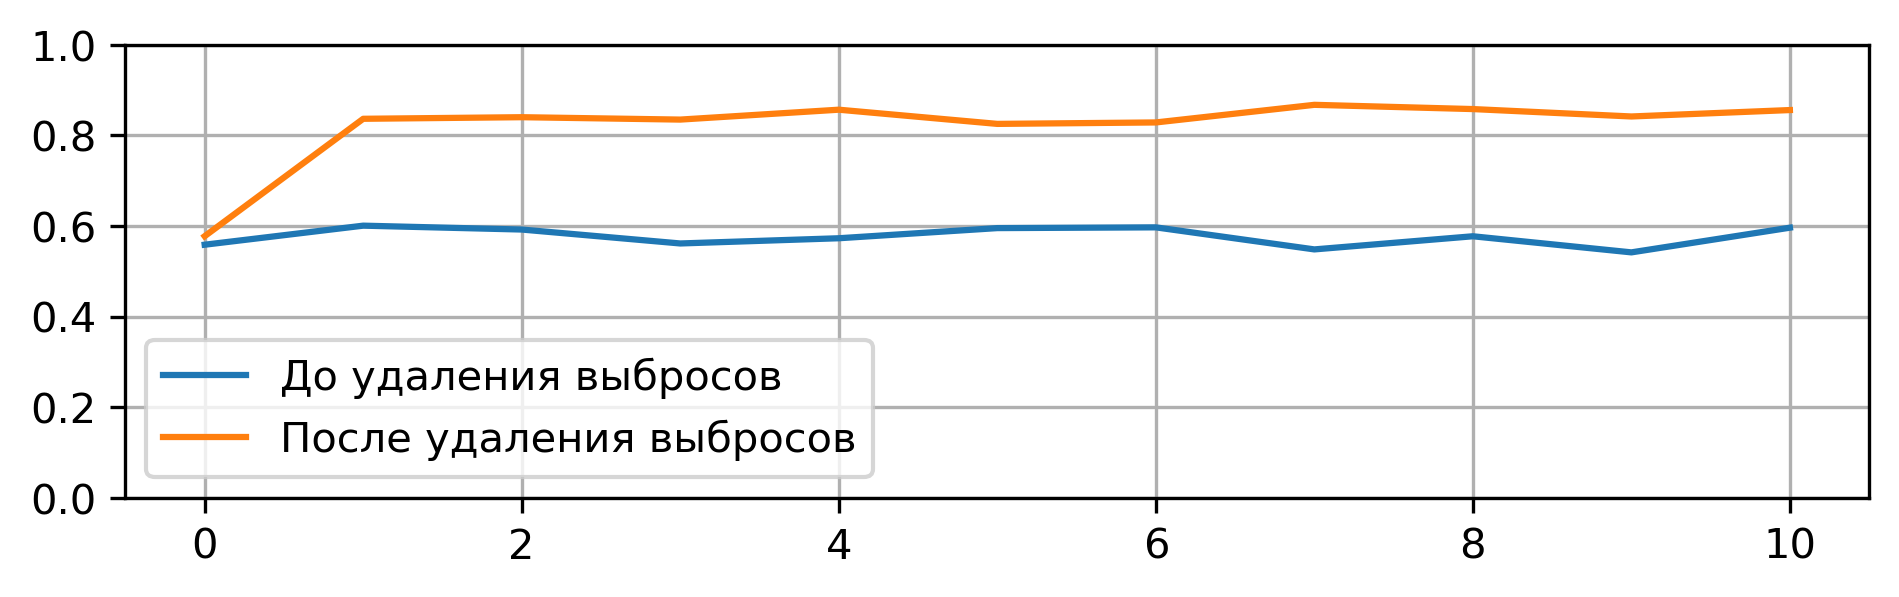
\includegraphics[width=0.8\linewidth]{pictures/Просмотры}
	\caption{Целевая функция 'Просмотры'}
\end{figure}
Поведение кривой коэффициента детерминации таково, что достаточно пожертвовать 1\% обучающих данных для качественного повышения производительности регрессионной модели. Дальнейшее увеличения числа отбракованных объектов не приводит к росту прогнозирующей способности.

\subsection{Целевая функция 'Показы'}

В целом, на этой целевой функции ситуация очень похожая. Процент объектов, которые мы готовы признать аномальными, изменяется от 0\% до 10\%. Коэффициент детерминации на неочищенных данных приблизительно постоянен и находится в районе 0.5. 

После удаления выбросов коэффициент детерминации находится в районе 0.7, и это тоже огромная разница в прогнозирующей способности моделей до и после удаления выбросов.

\begin{figure}[!h]
	\centering
	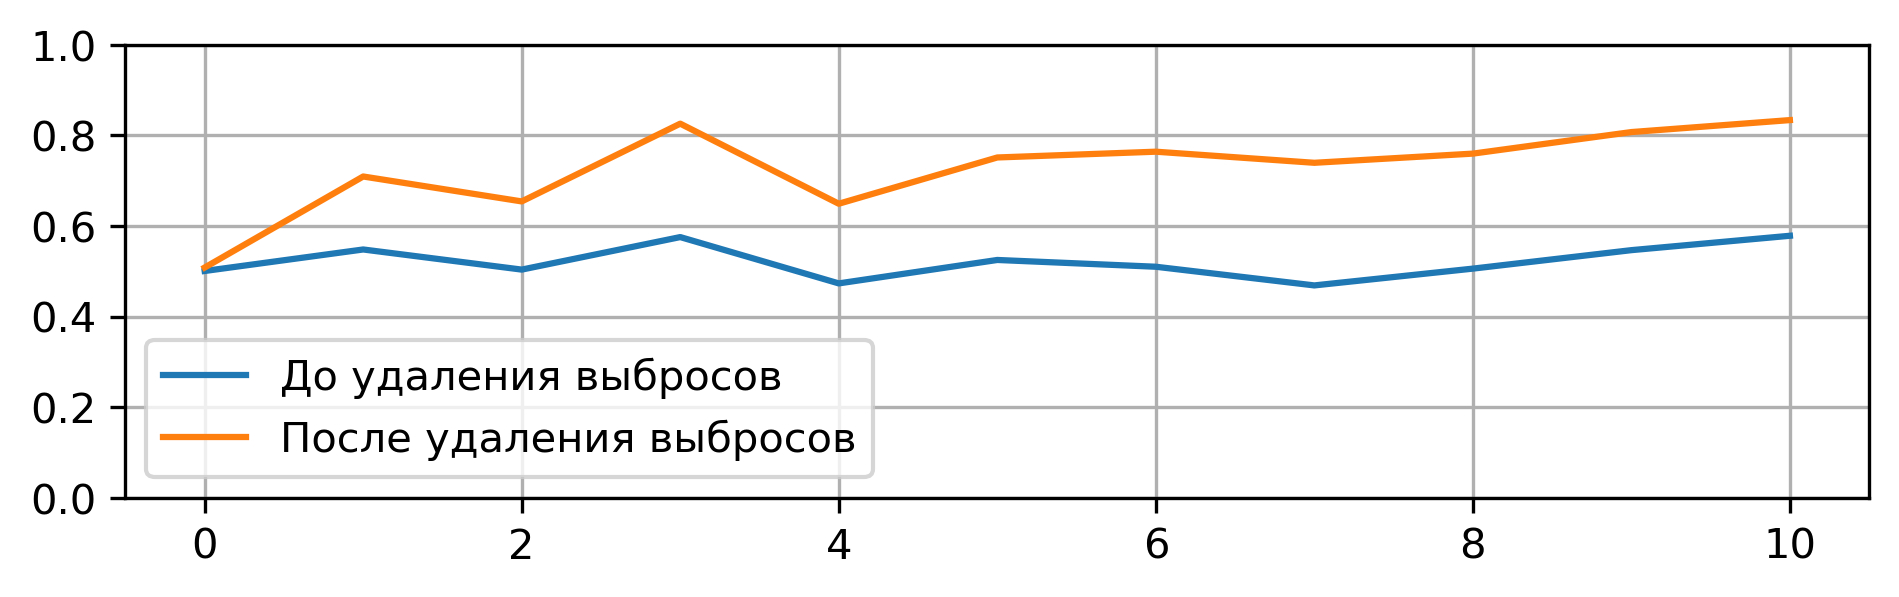
\includegraphics[width=0.8\linewidth]{pictures/Показы}
	\caption{Целевая функция 'Показы'}
\end{figure}


\subsection{Целевая функция 'Лайки'}

Здесь ситуация принципиально иная. Мы видим, что кривые коэффициентов детерминации практически совпадают (и видимо, при бесконечном увеличении числа прогонов совпадут до неразличимости), а это значит, что удаление выбросов никак не влияет на повышение прогнозирующей способности регрессионной модели.

\begin{figure}[!h]
	\centering
	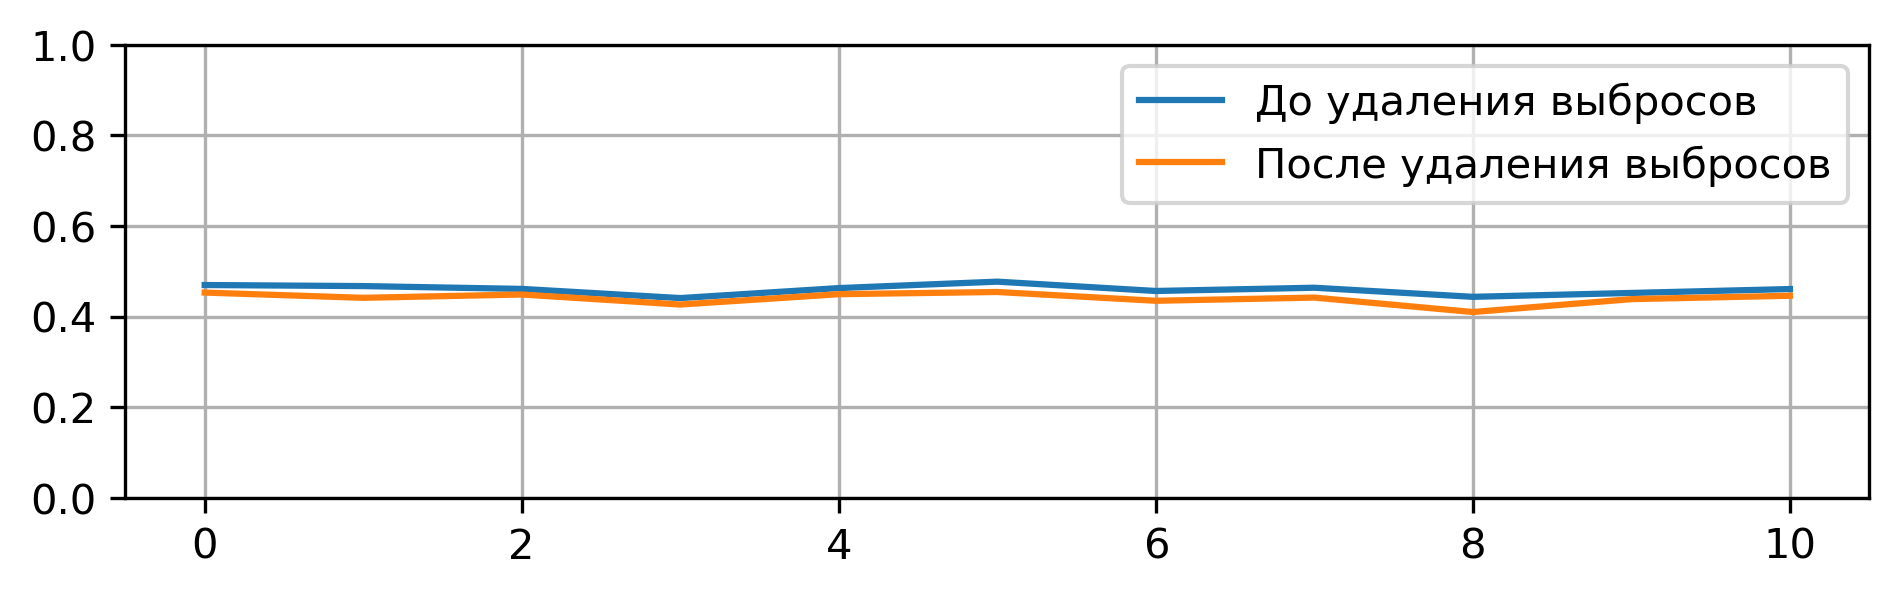
\includegraphics[width=0.8\linewidth]{pictures/Лайки}
	\caption{Целевая функция 'Лайки'}
\end{figure}

\section{Выводы}


Напомним принципы, сформулированные нами в самом начале, во введении к этой работе:

\medskip\noindent
\begin{enumerate}
	\item Обучать модели следует только на типичных объектах.
	\item Применять модели следует только к типичным объектам.
\end{enumerate}


\medskip\noindent
Соотнесем их с полученными результатами. С одной стороны, наши принципы не нашли своего подтверждения, так как мы выяснили, что они не универсальны, и возможны ситуации, когда удаление выбросов не приводит к повышению производительности (см. рис.~3). С другой стороны, возможны и оптимистичные сценарии (см. рис.~1 и~2). Поэтому будет верным скорректировать формулировку наших принципов, добавив к ним условие их справедливости:

\medskip\noindent
\begin{enumerate}
	\item Если исключение выбросов приводит к повышению производительности, то обучать модели следует только на типичных объектах.
	\item Если исключение выбросов приводит к повышению производительности, то применять модели следует только к типичным объектам.
\end{enumerate}


\medskip\noindent
Условие, при котором принципы очистки данных оказываются рабочими и эффективными методами моделирования, требуют предварительного анализа данных и не всегда проявляются. Но то, что есть ситуации, в которых удаление аномальных объектов приводит к существенному эффекту — несомненно.


\section{Литература}


\begin{enumerate}
	\item Хейдт М. Изучаем Pandas / М. Хейдт;  — Москва: ДМК Пресс, 2018. — 438 с. — ISBN 978-5-97060-625-4. — Текст: непосредственный.
	\item Бурков А. Машинное обучение без лишних слов / А. Бурков;  — СПб: Питер, 2020. — 192 с.
	\item Вьюгин, В. В. Математические основы теории машинного обучения и прогнозирования / В. В. Вьюгин; — М.: МЦИМО. — 2013. — 387~с.
	\item Бринк Х. Машинное обучение / Х. Бринк, Дж. Ричардс, М. Феверолф  — СПб.: Питер, 2017. — 336~с.
	\item Дрейпер Н. Р. Прикладной регрессионный анализ / Дрейпер Н. Р., Смит Г.; ред. пер. Саит-Аметова М.; Пер. с англ. и ред. пер. Власенко М., Имамутдинова Р. Г., Орехова Н. А., Саит-Аметова М. --- 3-е изд. --- М. : Диалектика : Вильямс, 2007. --- 911 с.
	\item Безменов И. В. Метод очистки измерительных данных от выбросов: поиск оптимального решения с минимальным количеством отбракованных результатов измерений // Измерительная техника. 2023. № 1. С. 16--23. 
	\item Безменов И. В., Дроздов А. Э., Пасынок С. Л. Стратегия поиска выбросов в рядах зашумлённых данных с неизвестным трендом // Измерительная техника. 2022. № 5. С. 29--34.
	\item Ахметшина Л.Г. Адаптивная фильтрация шумов методом сингулярного разложения автоморфного отображения // Вестник компьютерных и информационных технологий. 2006. № 8 (26). С. 12--21.
	\item Бурнашев Д.С., Залыгаева М.Е. Реализация рекомендательной системы пользовательских предпочтений на основе сингулярного разложения матриц на языке Python // В сборнике: Труды молодых учёных факультета компьютерных наук ВГУ. Сборник статей. Воронеж, 2023. С. 11--18.
\end{enumerate}


\end{document}